\documentclass[a4paper]{article}
\usepackage{array}  
\usepackage[table]{xcolor}% http://ctan.org/pkg/xcolor
\usepackage{geometry}
\geometry{margin=1.25in}
\usepackage{hhline}
\usepackage{environ}
\usepackage{graphicx}
 %\geometry{
 %a4paper,z
 %total={170mm,257mm},
 %left=40mm,
 %right=40mm
 %}
 \newcommand{\colWidth}{141mm}

\begin{document} 
\section*{Demo day: \textit{(demo 3)} Group \textit{(group 10)}}

% ------------GOALS----------

\begin{center}
\begin{tabular}{|p{\colWidth}|}
	\hline
	\cellcolor{blue!25}\large
	\textbf{What were your goals?}
	\\ \hline
	\vtop to 95mm{
\begin{itemize}
    \item B.O.B Hardware
    \begin{itemize}
         \item Finalise B.O.B grabber. 
         \item Improve B.O.B lift. 
    \end{itemize}
    \item B.O.B Software
    \begin{itemize} 
        \item Improve B.O.B sideways movement.
        \item Implement B.O.B grabbing.
        \item Connecting Pi and EV3, to server via SDP\_AT.
    \end{itemize}
    \item Server: 
    \begin{itemize}
        \item Expanded functionality; host on Heroku (Cloud hosting).
    \end{itemize}
    \item App:
    \begin{itemize}
        \item User QR Code Generation.
        \item UI enhancement.
    \end{itemize}
    \item Website: 
    \begin{itemize}
        \item UI enhancement.
        \item Finalise B.O.B has Logo.
        \item QR Code scanning.
    \end{itemize}
\end{itemize}
  }
  \\
  %have database - connects - get order and stuff - FOR SERVER
  \hline
\end{tabular}
\vskip 5mm

% ------------ORGANISATION----------

\begin{tabular}{|p{\colWidth}|}
	\hline
	\cellcolor{blue!25}\large
	\textbf{Summarise how your group organised the workload to achieve your goals.}
	\\ \hline
	\vtop to 95mm{
	\begin{itemize}
	    \item Team Split
	    \begin{itemize}
	        \item Robot Hardware
	        \item Robot Software
	        \item Server, Website and App 
	    \end{itemize}
	    \item Robot Hardware
	    \begin{itemize}
	        \item Jacob, Anna built B.O.B's grabber.
	        \item Jacob improved lift mechanism.
	    \end{itemize}
	    \item Robot Software
	    \begin{itemize}
	        \item Claire and Alex worked on grabbing (Freddie assisted). 
	        \item Claire and Alex improved sideways movement.
	    \end{itemize}
	    \item Server, Website and App 
	    \begin{itemize}
	        \item Freddie secured the connection between raspberry pi, EV3 and server. 
	        \item Oktay improved the App. Server testing, continuous integration and deployment for website and server. 
	        \item Kieran worked on QR Code Generation.
	        \item Harry improved the Website. Added server and website to the cloud (Oktay assisted).
	    \end{itemize}
	\end{itemize}
  }
  \\
  \hline
\end{tabular}
\vskip 5mm

% ------------ACHIEVEMENTS----------

\begin{tabular}{|p{\colWidth}|}
	\hline
	\cellcolor{blue!25}\large
	\textbf{What were your main achievements?}
	\\ \hline
	\vtop to 30mm{
	\begin{itemize}
	    \item B.O.B can grab.
	    \item Connection between EV3, raspberry pi to server is faster and reliable.
	    \item B.O.B sideways movement is improved.
	    \item App and Website integration.
	    \item Travis worked efficiently.
	\end{itemize}
  }
  \\
  \hline
\end{tabular}
\vskip 5mm

% ------------NOT ACHIEVED----------

\begin{tabular}{|p{\colWidth}|}
	\hline
	\cellcolor{blue!25}\large
	\textbf{What did you not achieve? Briefly explain why.}
	\\ \hline
	\vtop to 5mm{
	\begin{itemize}
	    \item Achieved goals.
	\end{itemize}
  }
  \\
  \hline
\end{tabular}
\vskip 5mm

% ------------NEXT STEPS----------

\begin{tabular}{|p{\colWidth}|}
	\hline
	\cellcolor{blue!25}\large
	\textbf{Say briefly what changes you will make to your plan for the next demo.}
	\\ \hline
	\vtop to 30mm{
	\begin{itemize}
	    \item Finalising B.O.B lift system.
	    \item HCI tests.
	    \item Unit tests for Website and App. 
	    \item More integration tests for Server.
	    \item Adding descriptive content to Website. 
	\end{itemize}
  }
  \\
  \hline
\end{tabular}

% ------------QUANTITIVE----------
\newpage
\begin{tabular}{|p{\colWidth}|}
	\hline
	\cellcolor{blue!25}\large
	\textbf{Include any quantitative data you have collected (this can be a graph/table with a few words)}
  \\
  \hline
\end{tabular}

\begin{figure}[!htb]
\minipage{0.90\textwidth}
  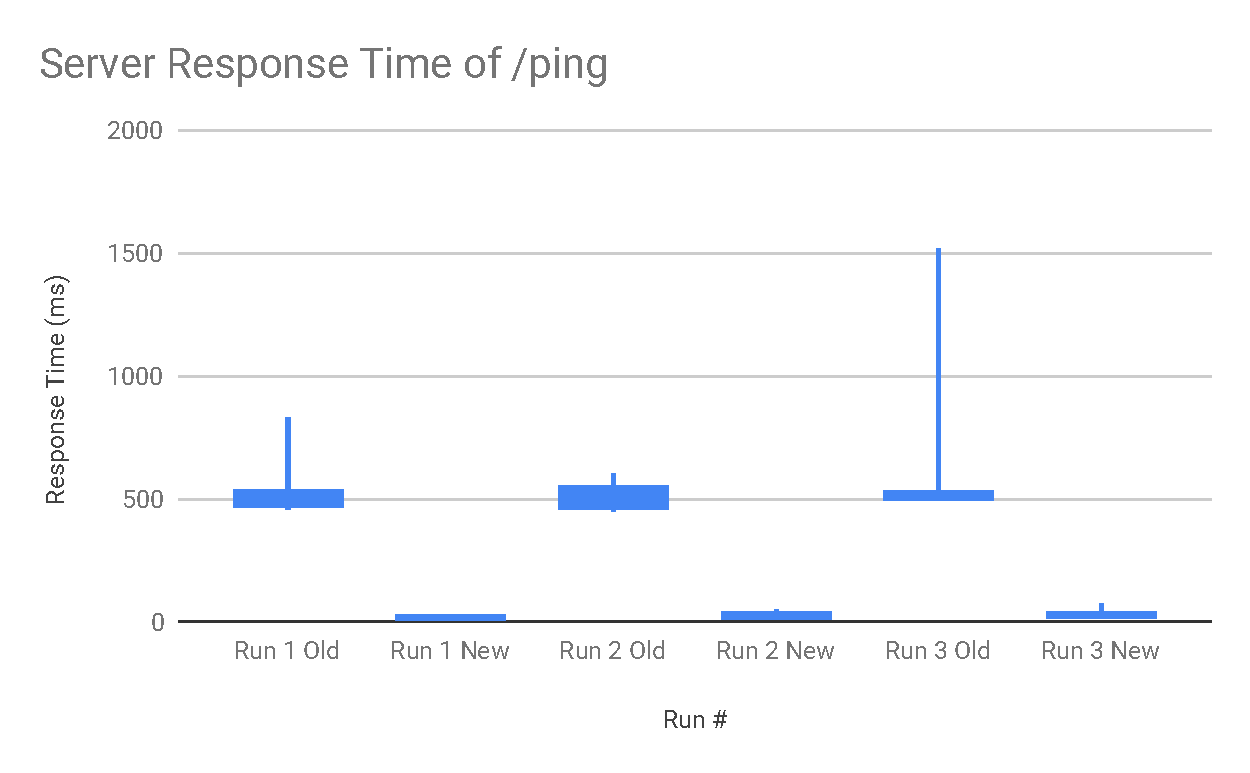
\includegraphics[width=\linewidth]{serv_resp.pdf}
  \caption{Difference between old (EV3) and new (Raspberry Pi) server response readings (on SDP\_AT).}\label{fig:awesome_image1}
\endminipage\hfill
    \minipage{0.90\textwidth}
     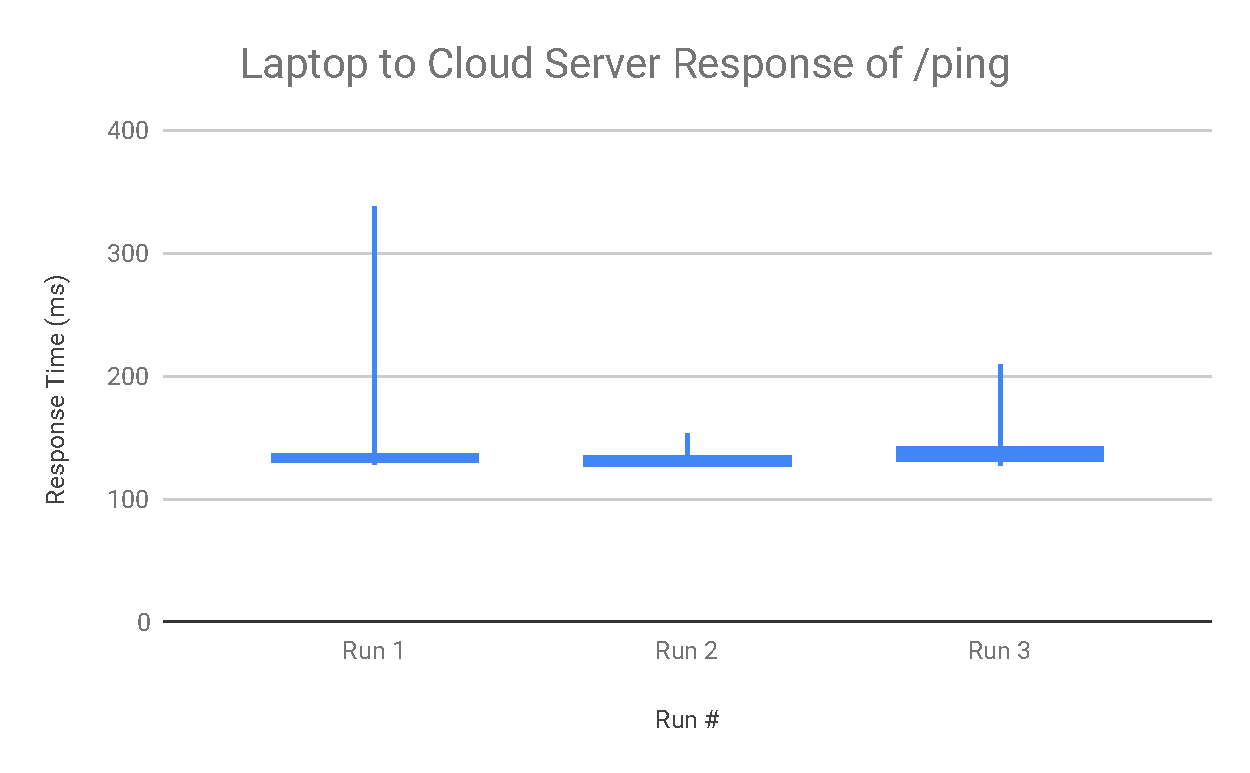
\includegraphics[width=\textwidth]{lap_serv.pdf}
     \caption{Laptop to server response readings.}\label{fig:awesome_image2}
\endminipage
\newline
\end{figure}

\begin{table}[!htb]
\centering
\begin{tabular}{| p{2cm} | p{2cm} | p{2cm} | p{2cm} |}
\hline
\textbf{Item} & \textbf{Cost Per Unit} & \textbf{Quantity} & \textbf{Total Cost} \\
\hline
EV3 Colour Sensor & £30.00 & 2 & £60.00 \\
\hline
Omni Wheels & £6.60 & 6 & £39.60 \\
\hline
Hardboards & £14.00 & 2 & £28.00 \\
\hline
Hypothetical Server Cost & £20.00 & 1 & £20.00 \\ 
\hline
 &  & \textbf{Total} & £147.60 \\ 
\hline
 &  & \textbf{Balance} & £52.40 \\
\hline
\end{tabular}
\caption{Finance}
\end{table}

\newpage
\begin{table}[!htb]
\centering
\begin{tabular}{| p{2cm} | p{2cm} |}
\hline
\textbf{Battery (mAh)} & \textbf{Voltage} \\
\hline
2200 & 7.5V \\
\hline
\end{tabular}
\caption{EV3 Battery and Voltage}
\end{table}

\begin{table}[!htb]
\centering
\begin{tabular}{| p{2cm} | p{2cm} | p{2cm} | p{2cm} | p{2cm} |}
\hline
\textbf{Component} & \textbf{Amperes (7.5V)} & \textbf{Number on Boards} & \textbf{Total Amperes} & \textbf{Total mA}\\
\hline
Colour Sensor & 0.107 & 4 & 0.428 & 428 \\
\hline
Motor (100\% running free) & 0.186 & 5 & 0.930 & 930 \\
\hline 
Processor (Full load) & 0.098 & 1 & 0.098 & 98 \\
\hline
 & & & \textbf{Battery Time From Full Charge (Hours)} & 1.511 \\ 
 \hline
\end{tabular}
\caption{Source https://www.dexterindustries.com/ev3-current-consumption-measurement/}
\end{table}

\begin{table}[!htb]
\centering
\begin{tabular}{| p{2cm} | p{2cm} | p{2cm} | p{2cm} | p{2cm} |}
\hline
\textbf{Component} & \textbf{Amperes (7.5V)} & \textbf{Number on Board} & \textbf{Total Amperes} & \textbf{Total mA}\\
\hline
Colour Sensor & 0.107 & 4 & 0.428 & 428 \\
\hline
Motor (100\% locked) & 0.911 & 5 & 4.555 & 4555 \\
\hline 
Processor (Full load) & 0.098 & 1 & 0.098 & 98 \\
\hline
 & & & \textbf{Battery Time From Full Charge (Hours)} & 0.433 \\ 
 \hline
\end{tabular}
\caption{Source https://www.dexterindustries.com/ev3-current-consumption-measurement/; locked implies lot of friction on motor}
\end{table}

\begin{table}[!htb]
\centering
\begin{tabular}{| p{2cm} | p{2cm} | p{2cm} | p{2cm} | p{2cm} |}
\hline
\textbf{Component} & \textbf{Amperes (7.5V)} & \textbf{Number on Board} & \textbf{Total Amperes} & \textbf{Total mA}\\
\hline
Phigit & 0.5 & 1 & 0.5 & 500 \\
\hline
Servo & 0.18 & 1 & 0.18 & 180 \\
\hline 
Raspberry Pi & 1.2 & 1 & 1.2 & 1200 \\
\hline
 & & & \textbf{Battery Time From Full Charge (Hours)} & 2.872 \\ 
 \hline
\end{tabular}
\caption{Source: Data provided by manufacturers}
\end{table}

\begin{table}[!htb]
\centering
\begin{tabular}{| p{2cm} | p{2cm} | p{2cm} | p{2cm} | p{2cm} |}
\hline
\textbf{Component} & \textbf{Amperes (7.5V)} & \textbf{Number on Board} & \textbf{Total Amperes} & \textbf{Total mA}\\
\hline
Small Motor & 0.202 & 1 & 0.202 & 202 \\
\hline
 & & & \textbf{Battery Time From Full Charge (Hours)} & 102.970\\ 
 \hline
\end{tabular}
\caption{Source: Data provided by manufacturers}
\end{table}

\end{center}
  
\end{document}
